\documentclass{article}
\usepackage[pdftex]{graphicx}
\usepackage{url}
\author{Rohit Kumar \\UCLA ID: 203884129}
\title{Data Mining Chess Games \\ CS 249: Term Project, Winter 2011}
\begin{document}


\maketitle


\section{Introduction}
\label{sec:intro}
The Free Internet Chess Server (FICS) \footnote{http://www.freechess.org} maintains an extensive set of chess games in its database. The data set contains games from 1999 to 2011 and includes players of all kinds of ratings -- from the very beginner, to grand masters, to computers. Apart from the traditional chess games, people also play chess variants on the server. For example: suicide chess, losers, crazhouse etc. The data for each game is captured as a Portable Game Notation (PGN) \cite{wiki:pgn} file and contains information regarding the moves played, the players names, their rating, time controls used and the result. \\

As of this writing the FICS chess database contains game records for over 130,000,000 chess games, played by over 300,000 humans and 1,400 computers. This project aims at finding interesting patterns in the FICS chess data set.

\section{PGN Parser}

As mentioned in Section~\ref{sec:intro}, the games in the FICS
database are stored in the PGN file format. PGN is a standard way for
storing chess games. It was designed for ease of viewing of chess
games and not for querying ~\cite{spec:pgn}. Thus to extract meaningful information out of the database, the PGN files need to be parsed.

PGN is a text based format and looks in some ways similar to the Windows INI file format. An example file, is shown in Figure~\ref{fig:pgn}

\begin{figure}[tph]
\begin{center}
\begin{verbatim}
[Event "FICS rated blitz game"]
[Site "FICS"]
[FICSGamesDBGameNo "273548609"]
[White "tirsa"]
[Black "EyeLikePie"]
[WhiteElo "1015"]
[BlackElo "1083"]
[TimeControl "180+0"]
[Date "2011.03.01"]
[Time "18:00:00"]
[WhiteClock "0:03:00.000"]
[BlackClock "0:03:00.000"]
[ECO "C57"]
[PlyCount "33"]
[Result "1-0"]


1. e4 {[%emt 0.0]} e5 {[%emt 0.0]} 
2. Nf3 {[%emt 0.57]} Nc6 {[%emt 0.39]} 
3. Bc4 {[%emt 0.692]} Nf6 {[%emt 2.781]} 
4. Ng5 {[%emt 1.812]} d5 {[%emt 7.405]} 
5. exd5 {[%emt 1.79]} Nxd5 {[%emt 0.859]} 
6. Qf3 {[%emt 6.995]} Qxg5 {[%emt 11.124]} 
7. Bxd5 {[%emt 2.384]} f6 {[%emt 14.233]} 
8. Bxc6+ {[%emt 3.291]} bxc6 {[%emt 1.796]} 
9. d3 {[%emt 1.242]} Bb4+ {[%emt 1.719]} 
10. Nc3 {[%emt 3.945]} Bxc3+ {[%emt 4.969]} 
11. bxc3 {[%emt 1.391]} Qg6 {[%emt 4.593]} 
12. O-O {[%emt 5.834]} Bg4 {[%emt 0.672]} 
13. Qxc6+ {[%emt 4.156]} Kf7 {[%emt 3.172]} 
14. Qxc7+ {[%emt 0.899]} Ke6 {[%emt 2.343]} 
15. Qc4+ {[%emt 1.71]} Kf5 {[%emt 4.203]} 
16. f3 {[%emt 0.733]} Bxf3 {[%emt 1.828]} 
17. Rxf3# {[%emt 3.97]} {Black checkmated} 1-0

\end{verbatim}
\end{center}
\caption{Example PGN File.}
\label{fig:pgn}
\end{figure}

Each PGN file can have details regarding more than one game. A game contains some meta information like the player information, their ratings, the time controls used, which is followed by the actual moves played by the players.\\

The meta information is stored as key-value players and are the fields enclosed within '[' and ']' in Figure ~\ref{fig:pgn}. The moves come after that and are prefixed with numbers. The white player's move is listed first, followed by black. The moves are denoted using the Standard Algebraic Chess Notation ~\cite{wiki:san}. \\

The PGN parser extracts both the meta information and the moves from the PGN file. The contents of the entire PGN file is stored within a \verb=PgnDatabase= class. The \verb=PgnDatabase= class contains a list of \verb=PgnGame= instances.

\section{Player Statistics}
\label{sec:pstats}
The PGN database only gives details regarding individual games played on the FICS server. It doesn't give us individual player statistics. These were gathered by executing a command on the FICS server called \verb=finger=. 

The \verb=finger= command lists a player's details such as, their rating, number of games played, won, lost, etc. An example output of running the command \verb="finger roxtar"= on the FICS server is shown in Figure ~\ref{fig:finger}

\begin{figure}[tph]
\begin{verbatim}
>finger roxtar

Finger of roxtar:

On for: 29 mins   Idle: 0 secs

          rating     RD      win    loss    draw   total   best
Blitz      1044     34.2     670     693      30    1393   1161 (04-Apr-2008)
Standard   1178    350.0       3       5       0       8
Lightning  1004    289.5       5      10       0      15
Bughouse   1323    350.0       2       4       0       6
Crazyhouse 1388    166.7      16      26       0      42   1272 (27-Feb-2005)
Suicide    1705    173.5     152     222       6     380   1654 (08-Dec-2004)
Losers     1877    350.0       7       6       0      13


Timeseal 1 : On

 1: I prefer 2 12 or 10 0.
 2: No takebacks asked or given.
 3: The variants which I like to play include suicide and crazyhouse.
\end{verbatim}
\caption{Example Finger Output}
\label{fig:finger}
\end{figure}

\pagebreak

To execute the \verb=finger= command on the server a Perl script was written, which would telnet to the FICS server, run the command and return the output \footnote{The finger command can also be executed from the FICS website. In fact the initial method to obtain player statistics used the website. A script would repeatedly query the website for the statistics. This method though generated a lot of requests for the web server and server administrators blocked the author's IP address from accessing the web page.}  The output was then filtered to obtain the player statistics in CSV format. \\

The FICS website or server doesn't provide a means to extract a list of all user names in the system. So instead, a PGN file containing 5000 games was downloaded for each month between March 2010 to March 2011 and the statistics for all users who participated in those games was extracted. 

\section{Exploring Ratings}
The FICS server has got a rating system based on the Glicko system ~\cite{spec:glicko}. Each player has a rating which is a number ranging between 600-3000. The higher the rating, the better the player. The Glicko rating system has another factor called \textsl{Ratings Deviation(RD)}, which measures the accuracy of the rating. The lower the Ratings Deviation (RD), the more accurate is the rating of the player.\\

In addition to this, the FICS server allows to users to play at a pace of their own choice. This leads to three varieties of time controls in regular chess: lightning, blitz and standard. Lighting being the fastest, with games finishing in under 6 minutes total, and standard being the slowest. For each of these different time controls, the user has different ratings, i.e a user's blitz rating will not be influenced by any of the lightning games which she plays and vice-versa.Time controls which fall under the blitz category are the most popular.\\

To explore the ratings of the players on FICS, the finger statistics were downloaded and transformed into a CSV format as described in section ~\ref{sec:pstats}. This was done separately for human players and computer programs. On plotting the histogram of the human ratings, for blitz games, we observe that the ratings have normal distribution (Figure \ref{fig:humanrating}). With the mean $\bar{x}_{hr} = 1339.560$ and standard deviation $\sigma_{hr} = 293.12$\footnote{The author's own rating is below average at 1084}.\\

\begin{figure} [tph]
\begin{center}
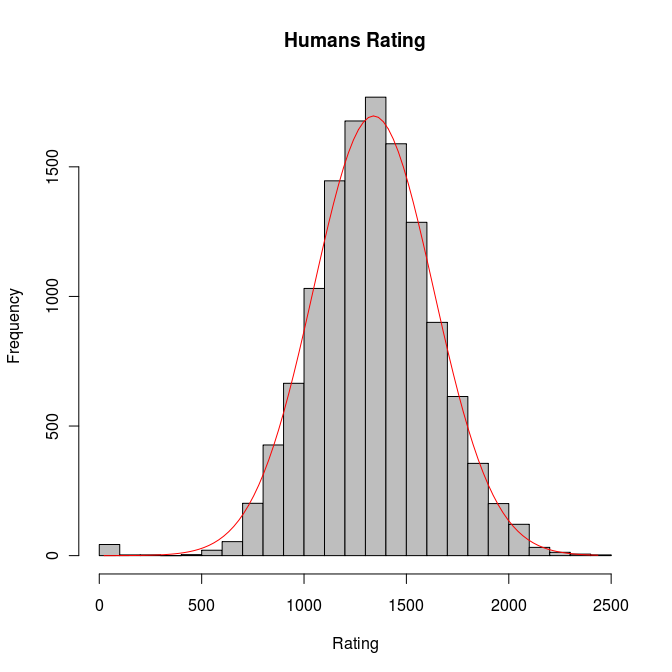
\includegraphics[width=3in]{humans_rating.png}
\end{center}
\caption{Distribution of Human Players' Rating}
\label{fig:humanrating}
\end{figure}


The list of computers operating on the FICS server was available readily. The same procedure was applied to obtain their statistics. The computer blitz ratings histogram differ significantly from the human ratings. We see in Figure \ref{fig:comprating} that the computer ratings do not seem to follow a normal distribution. Most computers are rated higher than 2000. To compare this against humans, $79.6\%$ of computers are rated above 2000, whereas only $1.44\%$ of humans cross that level. The mean rating for computers is $\bar{x}_{cr} = 2254.479$ with standard deviation $\sigma_{cr} = 426.53$. One thing to note though is that the number of active computer players is far less than human players.\\


\begin{figure} [tph]
\begin{center}
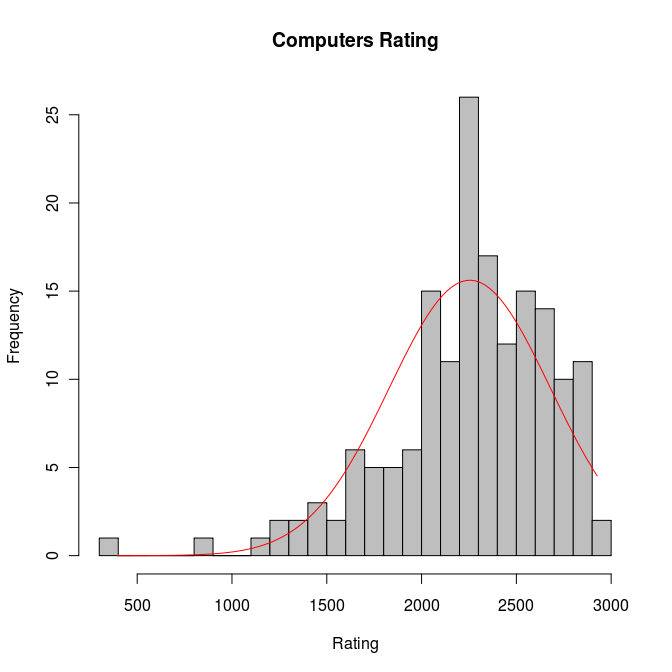
\includegraphics[width=3in]{computers_rating.png}
\end{center}
\caption{Distribution of Computers' Rating}
\label{fig:comprating}
\end{figure}

A related statistic is the number of games a particular user has played. One could conjecture that human players would have played lesser number of games as compared to the computers on the server. The totals for the blitz games played, were plotted for humans and computers (Figure ~\ref{fig:gametotals}). The computer which has played the highest number of blitz games is {\sl mscp(C)} and the human is a user named {\sl gianti}. What's surprising is that {\sl mscp(C)} has played over 1 million games, which is 10 times the number of games which {\sl gianti} has played.\\

Another thing which can be noticed is that most computers have totals below 200,000 games, whereas for humans this number is 60,000. We considered points above these numbers as outliers and plotted the histogram for the totals.

\begin{figure} [tph]
\begin{center}
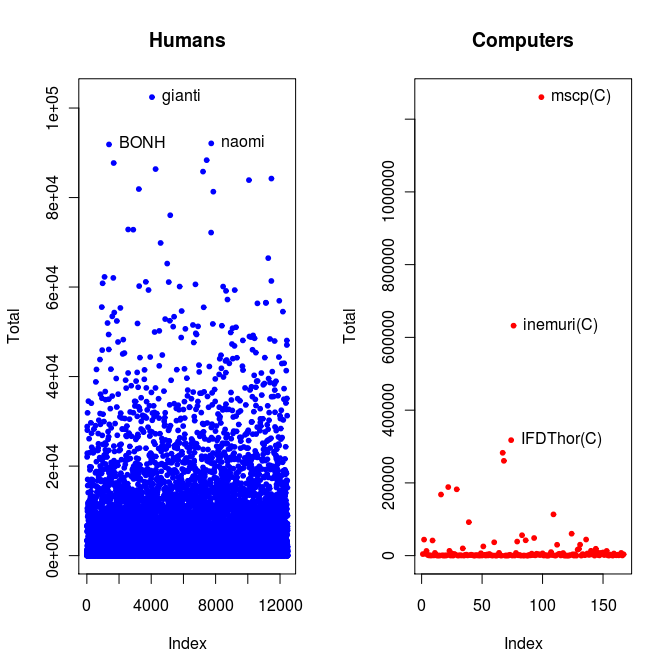
\includegraphics[width=3in]{game_totals.png}
\end{center}
\caption{Blitz Game Totals for Humans and Computers}
\label{fig:gametotals}
\end{figure}


\pagebreak
\bibliography{project_chess}
\bibliographystyle{plain}

\end{document}
